\documentclass{beamer}
\usepackage{graphicx}
\usepackage{tikz}
\usepackage[absolute,overlay]{textpos}
\usepackage{listings}
\usepackage{textpos}
%\usepackage{figlatex}
% \usetheme{default}
% \usetheme{Boadilla}
% \usetheme{Madrid}
% \usetheme{Montpellier}
\usetheme{Warsaw}
%\usetheme{Copenhagen}
% \usetheme{Goettingen}
% \usetheme{Hannover}
% \usetheme{Berkeley}

%\usecolortheme{crane}
%  \beamertemplatesolidbackgroundcolor{craneorange!25}

\title{Remote Robot Monitor}
\subtitle{Sistema di controllo e monitoraggio a distanza per robot mobili}

\author{Nicol\`o Grippaldi - Loris Fichera}

\institute[UniCT] {Universit\`a  degli Studi di Catania\\Corso di Laurea Specialistica in Ingegneria Informatica\\Corso di Sistemi Cognitivi e Interazione Uomo-Macchina}

\date[17 Febbraio 2009]
     {}
     
     \begin{document}
       
       
       \frame{
	 \titlepage
	 \begin{center}
	   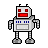
\includegraphics[width = 32 px]{images/Robot.png}
	 \end{center}
       }
       
%%descrizione del problema
% chi sono gli utenti
% quale e' il sistema con cui si deve interagire
% quale era lo schema di interazione precedente

%design
%  design dell'interazione
%  architettura dell'applicazione
%  spostamento della complessita' da una parte all'altra del sistema

%       \section[Outline]{}
       \frame{
	 \frametitle{Sommario}
	 %%A-RATIO LOGO
	 \tableofcontents
       }
       \section{Il dominio applicativo}         
       \begin{frame}
	     \frametitle{Eurobot Open 2009}
	     Eurobot Open 2009 \`e una competizione internazionale di robotica:\\
	     \begin{center}
	       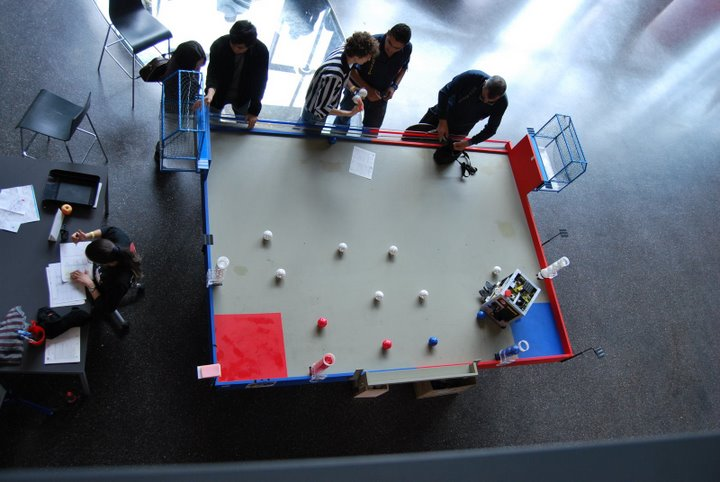
\includegraphics[width = 50.8mm]{images/eurobot.jpg}
	     \end{center}
	     \pause
	     \small 
	     I robot che vi prendono parte sono:
	     \begin{itemize}
	       \item \small mobili
	       \item \small intelligenti
	     \end{itemize}
	     \pause
	     \small
	     Prima della competizione, ogni squadra effettua numerosi test.
       \end{frame}

       \begin{frame}
	 \frametitle{Composizione di un team}
	 \begin{center}
	   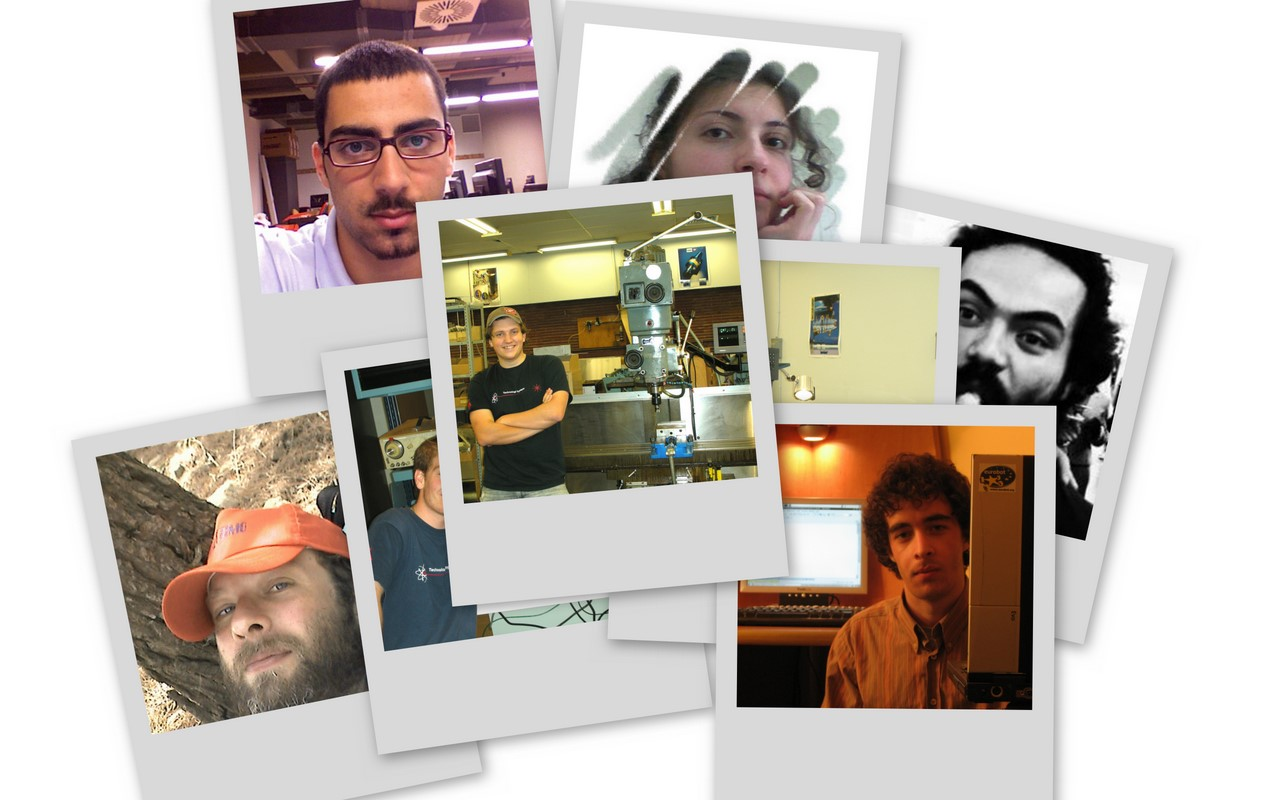
\includegraphics[width = 60mm]{images/collage.jpg}
	 \end{center}
	 I membri di un team sono, solitamente:
	 \pause
	 \begin{itemize}
	 \item Giovani non oltre i 30 anni di et\`a
	 \item Laureati in Ingegneria Elettronica/Informatica/Meccatronica
	 \item Esperti del dominio applicativo
	 \end{itemize}
       \end{frame}

       \begin{frame}
	 \frametitle{Il Robot}
	 \begin{center}
	   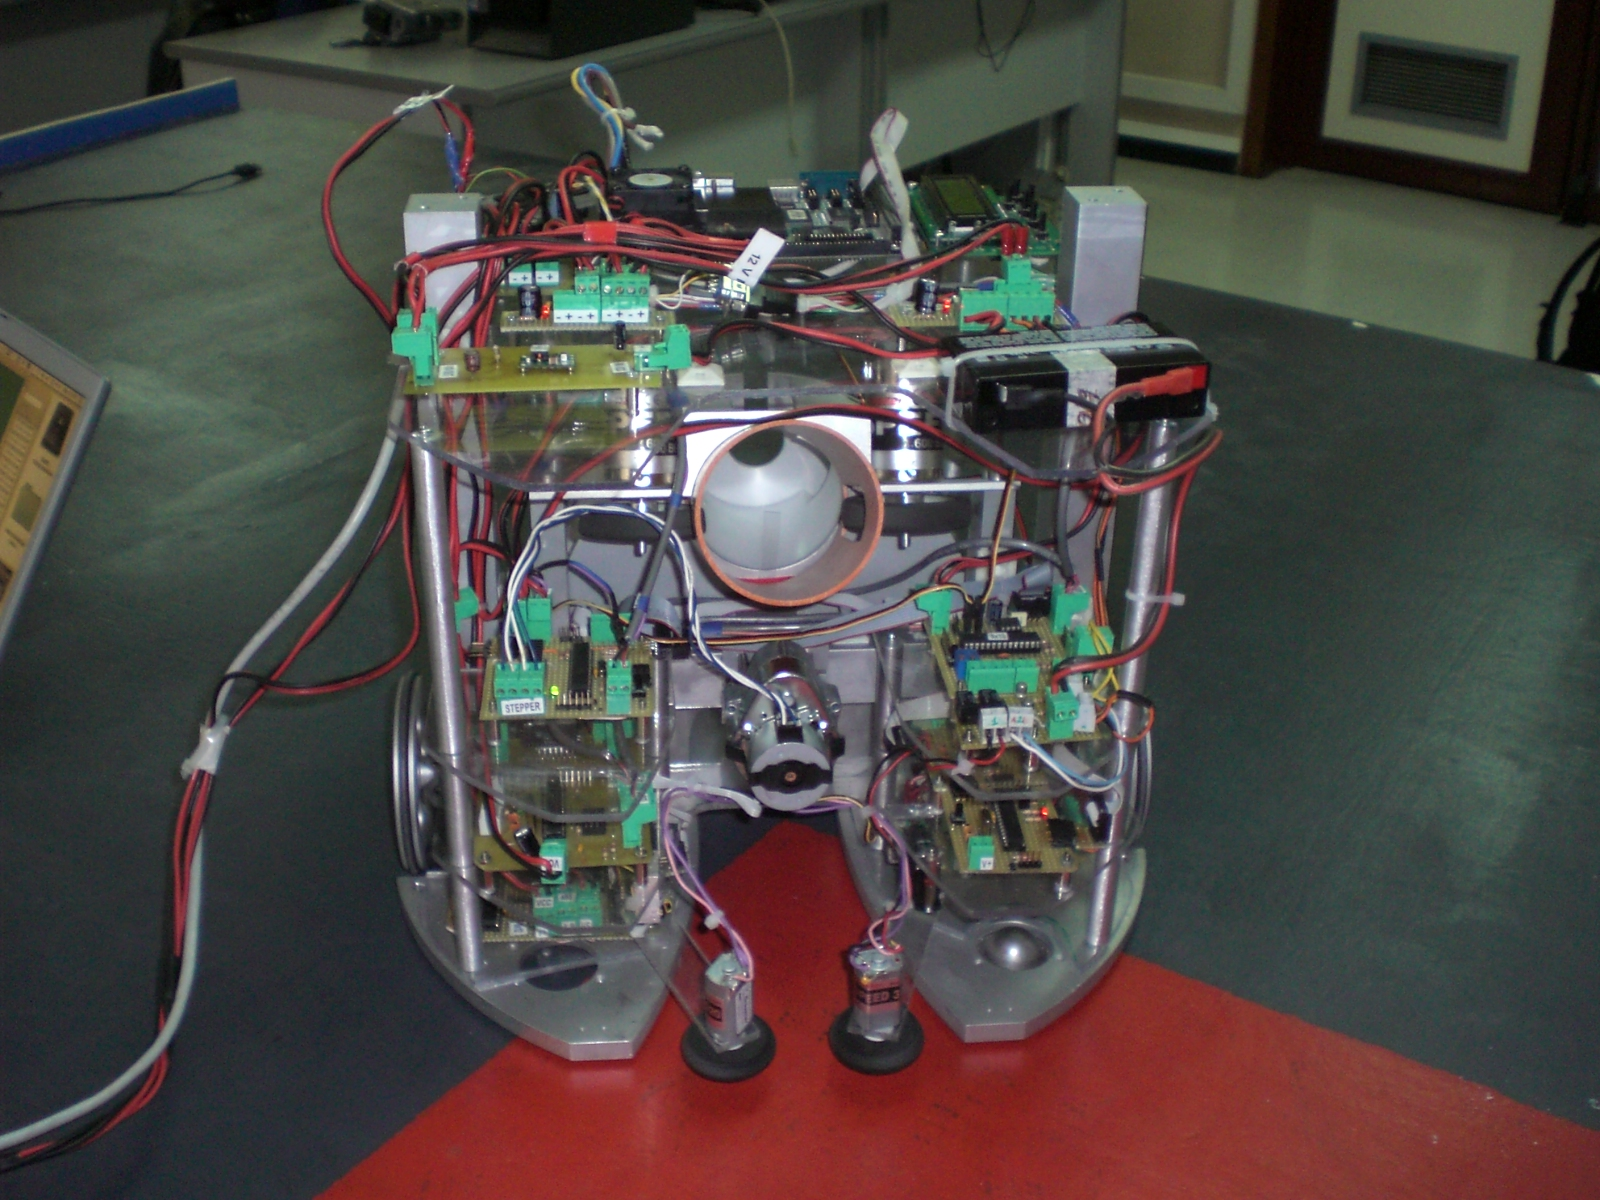
\includegraphics[width = 60mm]{images/robot.jpg}
	 \end{center}
	 \small Un robot \`e un sistema dotato di:
	 \pause
	 \begin{itemize}
	 \item \small Componenti meccaniche
	 \item \small Sensori
	 \item \small Intelligenza artificiale (framework robotico)
	 \end{itemize}
       \end{frame}

       \begin{frame}
	 \frametitle{Eseguire dei test: la struttura dell'interazione}
	 \begin{center}
	   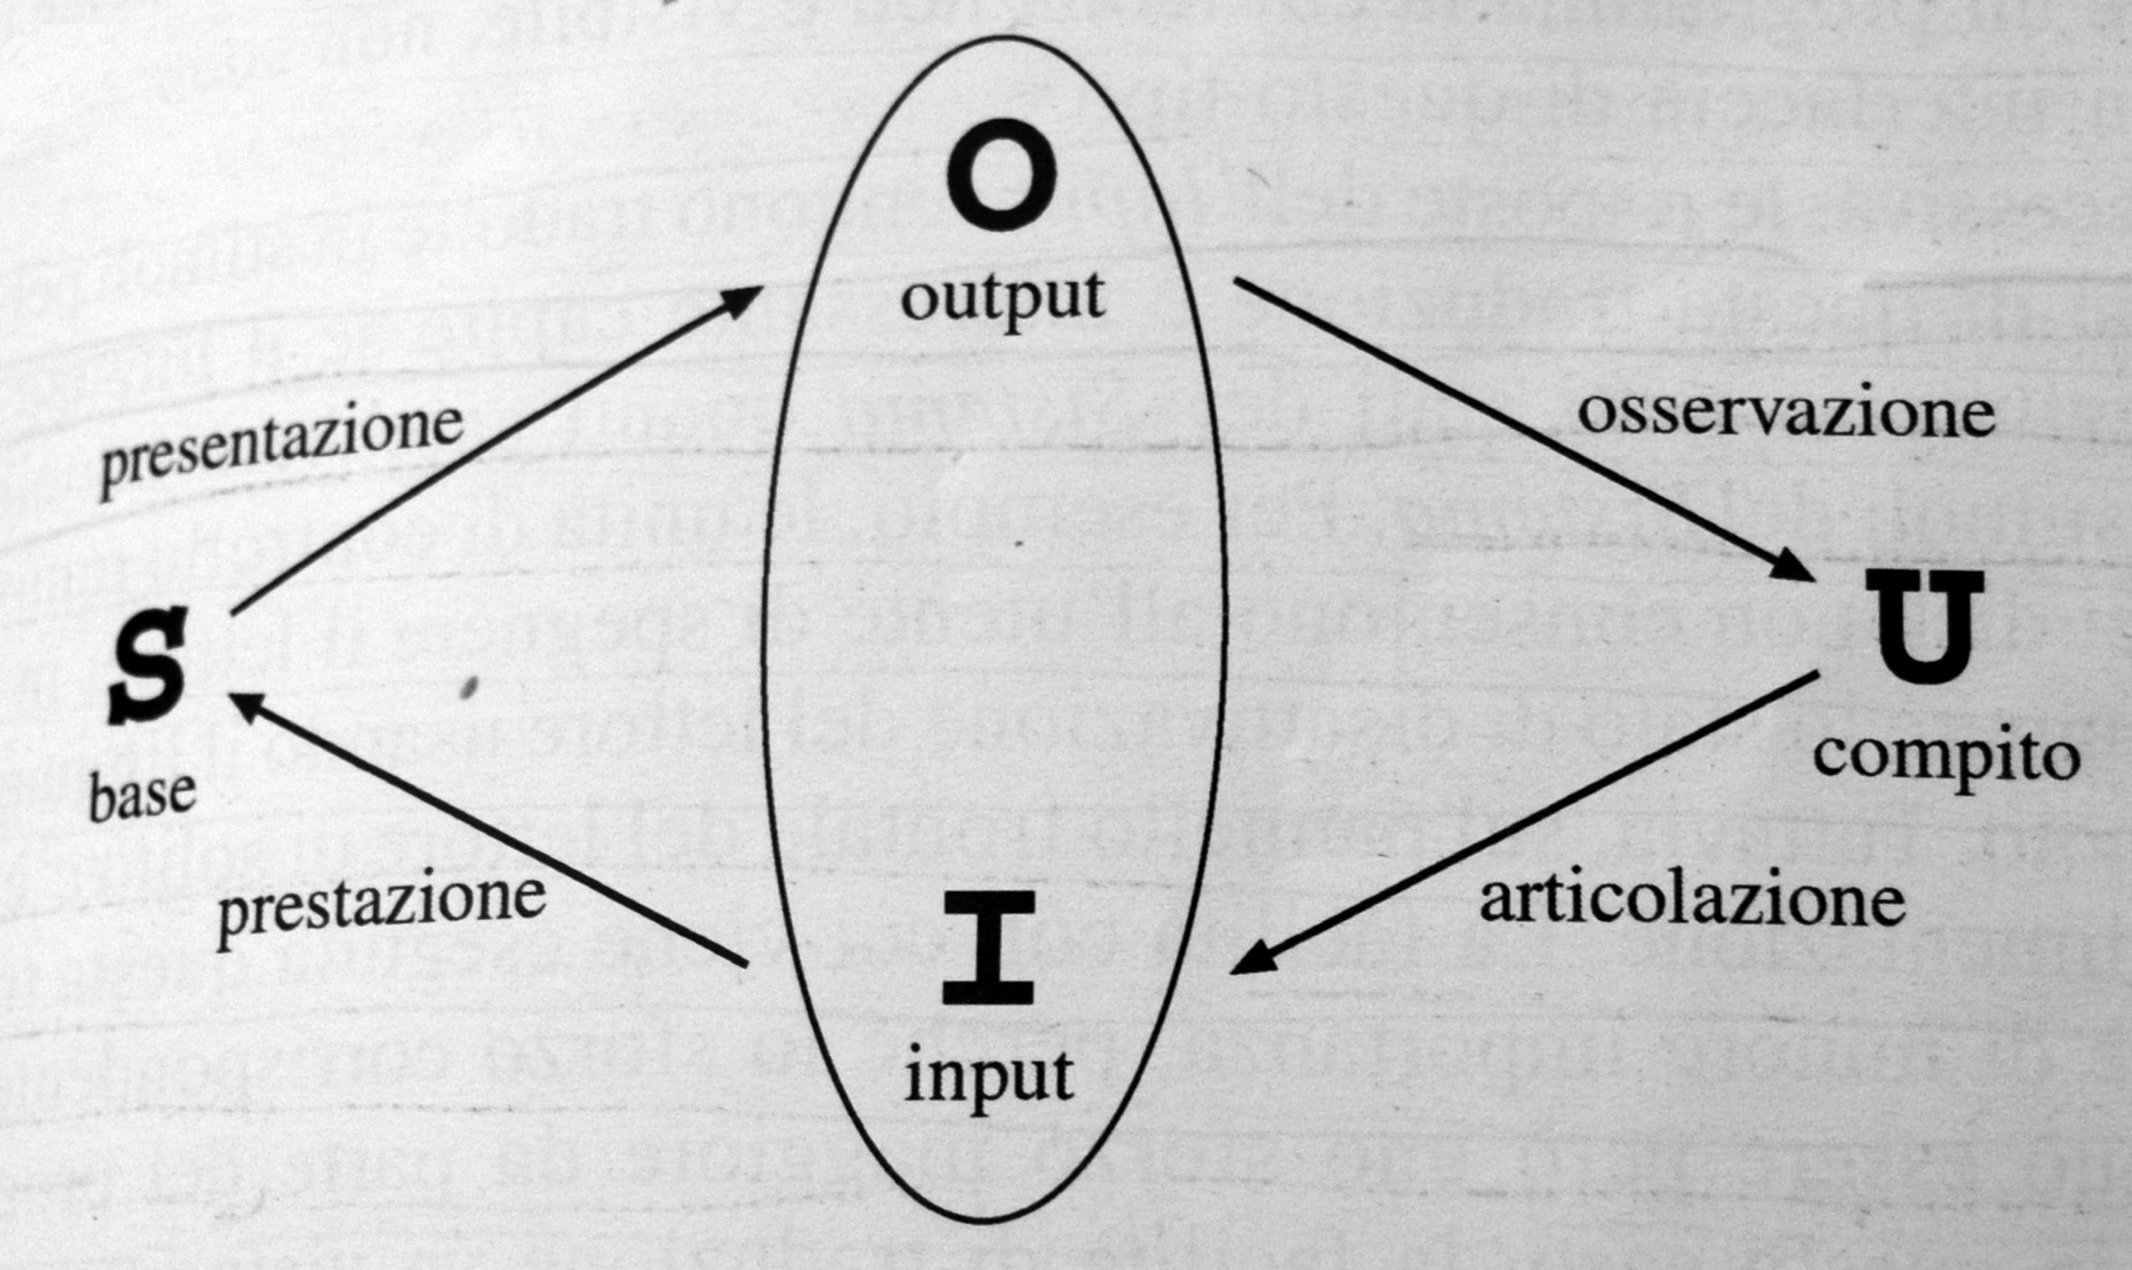
\includegraphics[width = 40 mm]{images/interaction_framework.jpg}
	 \end{center}
	 Per effettuare dei test \`e necessario pilotare manualmente il robot.
	 \newline
	 \pause
	 \begin{center}
	   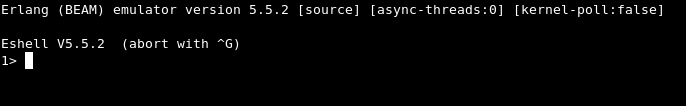
\includegraphics[width = 75 mm]{images/erl_shell.png}
	 \end{center}
	 L'interazione avviene a mezzo linea di comando, utilizzando la shell del linguaggio Erlang.
       \end{frame}

\section{Design dell'interazione}
       \begin{frame}
	 \frametitle{Re-Ingegnerizzazione dell'interazione / 1}
	 \begin{center}
	   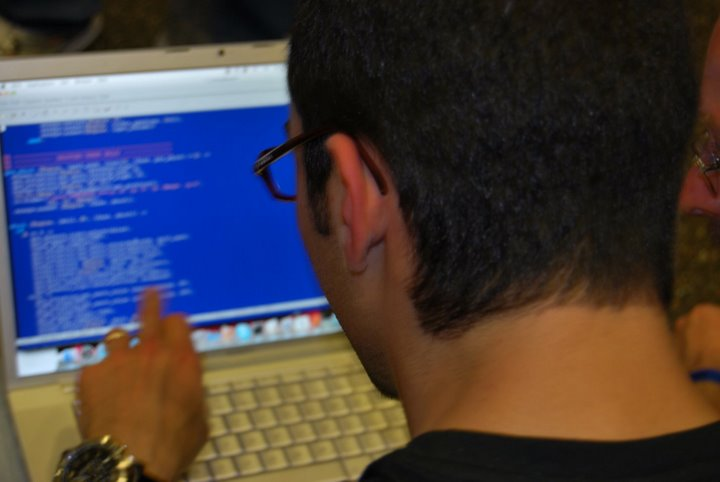
\includegraphics[width = 55mm]{images/command_line.jpg}
	 \end{center}
	 L'interazione a mezzo linea di comando \`e potente e flessibile, ma:
	 \begin{itemize}
	   \item Sovraccarica la working memory
	   \item Rende difficoltosa l'effettuazione di compiti ripetitivi
	   \item Obbliga l'utente a conoscere i comandi del framework robotico 
	 \end{itemize}
       \end{frame}

       \begin{frame}
	 \frametitle{Re-Ingegnerizzazione dell'interazione / 2}
\bf	 Legge di Tesler: 
\newline
{\bf \`e impossibile scendere al di sotto di una certa soglia di complessit\`a. L'unica opzione possibile \`e spostare la complessit\`a da una parte del sistema a un'altra.}
	 \pause
	 \newline
	 \newline
	 {\bf \`E quindi possibile introdurre un ulteriore livello di astrazione tra l'utente e il sistema e concentrarvi buona parte della complessit\`a.}
       \end{frame}

       \begin{frame}
	 \frametitle{RRM: architettura dell'applicazione / 1}
	 \small Lo stato dell'arte propone diverse possibili architetture per una applicazione basata su GUI.
	 \newline
	 \small Il pattern che meglio si adatta alle nostre esigenze \`e MVP (Model/View/Presenter).
	 \begin{center}
	   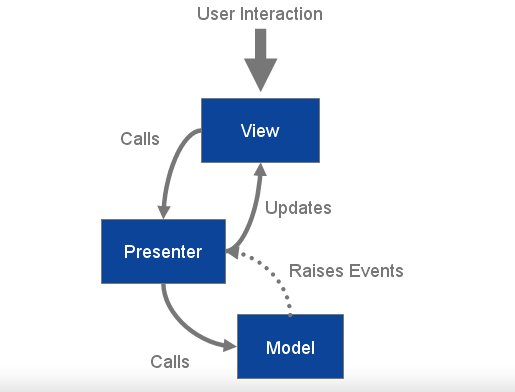
\includegraphics[width = 55mm]{images/mvp.jpg}
	 \end{center}
       \end{frame}

       \begin{frame}
	 \frametitle{RRM: architettura dell'applicazione / 2}
	 \begin{center}
	   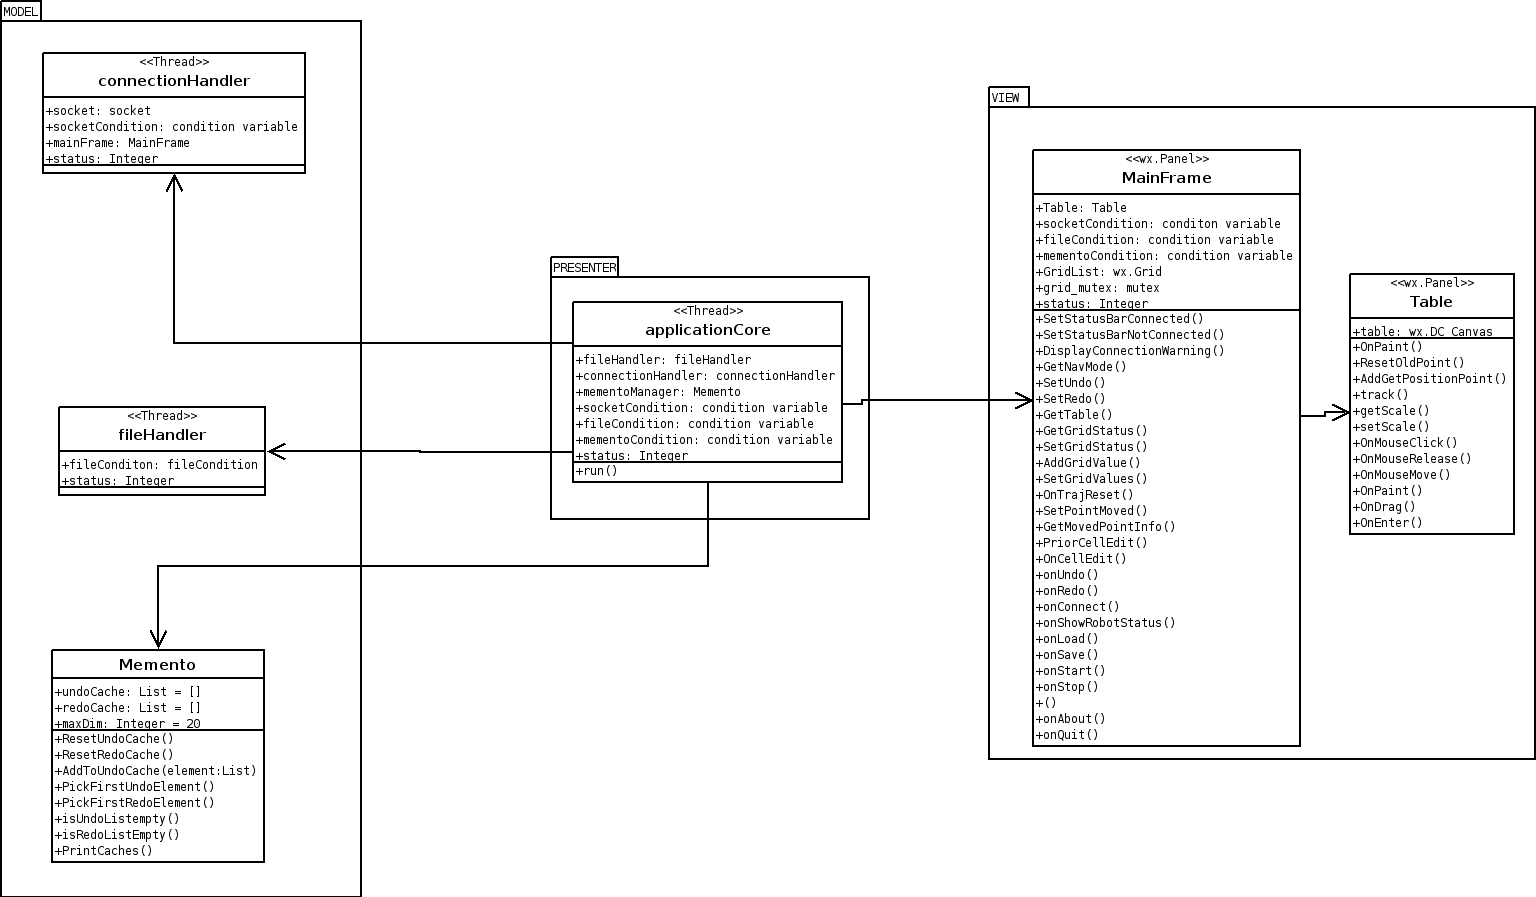
\includegraphics[width = 110mm]{images/classDiagram.png}
	 \end{center}
       \end{frame}

\section{Strumenti utilizzati}
       \begin{frame}
	 \frametitle{wxWidgets e wxPython}
	   
\includegraphics[width = 35mm]{images/wxWidgets.jpg}
	   \newline
	   {\bf wxWidgets}  \`e un framework {\it open source} per lo sviluppo di applicazioni multipiattaforma basate su GUI, in grado di fornire il {\it look and feel} nativo della singola piattaforma. \`E dotato di librerie per C++, compilatore e documentazione.
	   \pause
	   \newline
	   
\includegraphics[width = 35mm]{images/wxPython.jpg}
	   \newline
	   {\bf wxPython} \`e un modulo estensivo del linguaggio Python che incapsula classi e metodi forniti dalle librerie wxWidgets.
       \end{frame}
       \begin{frame}
	 \frametitle{wxGlade}
	 \begin{center}
	   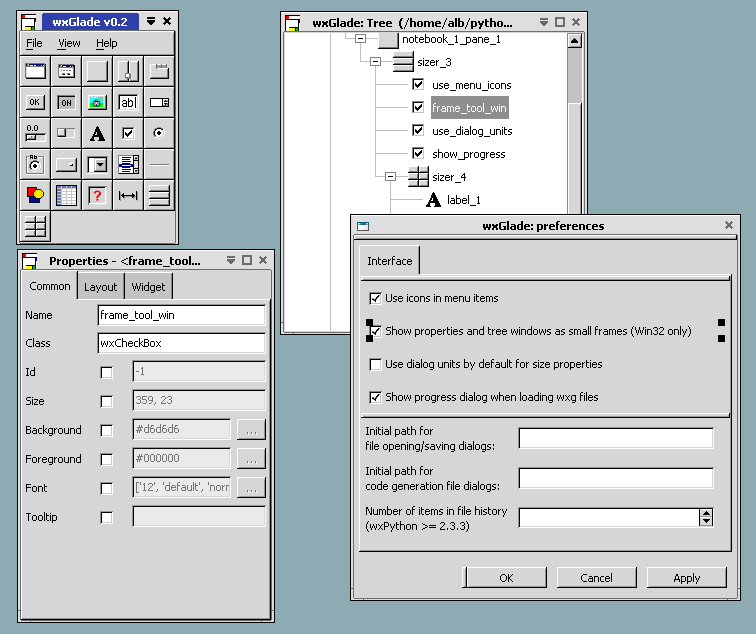
\includegraphics[width = 45mm]{images/wxglade.png}
	 \end{center}
  \small
	 {\bf wxGlade} \`e un designer grafico di GUI scritto in Python. Sfrutta il modulo wxPython. Il suo scopo \`e facilitare la creazione di widgets e interfacce utente. \`E in grado di generare codice Python, C++, Perl, Lisp.
       \end{frame}

\section{L'interfaccia}
\begin{frame}
  \frametitle{L'interfaccia}
\end{frame}

\section{Test d'Usabilit\`a}
\begin{frame}
\frametitle{Test d'Usabilit\`a}
  Il test d'usabilit\`a \`e stato condotto su due membri del team:
  \pause
  \medskip
  \begin{itemize}
  \item Carlo B.
    \newline
    \small 23 anni, studente di Ingegneria dell'Automazione
  \item Andrea M.
    \newline
    \small 24 anni, studente di Ingegneria Informatica
  \end{itemize}
\bigskip
\pause
\`E stato loro chiesto di effettuare i due seguenti compiti:
\begin{itemize}
  \item Test del sistema di Obstacle Avoidance
    \newline
    \begin{small} {\it Connettersi al Robot, impostare e fargli effettuare una traiettoria, controllare che il sistema di obstacle avoidance funzioni.}
      \end{small}
  \item Recupero e modifica di una sessione salvata
    \newline
    \begin{small} {\it Aprire una traiettoria salvata su file, modificare alcuni punti della traiettoria, quindi salvarla.}
    \end{small}
\end{itemize}
\end{frame}

\begin{frame}
\frametitle{Test del sistema di Obstacle Avoidance}
\begin{itemize}
  \item Carlo
    \newline
    \begin{tiny}
      Durante l'impostazione della traiettoria commette un errore. Nel menu ``Actions'', trover\`a la voce ``Undo'' e ripristiner\`a lo stato precedente. \newline Carlo trova rapidamente il modo per connettersi, a connessione avvenuta preme il pulsante ``Start'' e osserva ci\`o che succede. Carlo verifica il funzionamento del sistema di Obstacle Avoidance osservando la traiettoria bianca che va a tracciarsi sul tavolo e che descrive la traiettoria realmente effettuata dal robot. Infine, lamenta la mancanza di una rappresentazione visuale dello stato dei sensori di obstacle avoidance.
    \end{tiny}
  \item Andrea
\begin{tiny}
    \newline L'unica difficolt\`a \`e stata incontrata durante la fase di connessione con il robot in quando Andrea ha inserito un indirizzo non valido. Grazie all'aiuto di un messaggio di errore, \`e riuscito a capire dove ha sbagliato e quindi, successivamente, \`e riuscito a connettersi al robot.
    \end{tiny}
\end{itemize}
\end{frame}

\begin{frame}
\frametitle{Recupero e modifica di una sessione salvata}
\begin{itemize}
  \item Carlo
    \newline
    \begin{tiny}      
Carlo trova il compito agevole. Dopo aver caricato una traiettoria da noi precedentemente salvata su file, modifica alcuni punti via drag and drop. Il cambio di cursore in vicinanza dei punti, gli ha infatti suggerito tale possibilit�.
Al termine della modifica, salva la traiettoria utilizzando, istintivamente, la combinazione di tasti ``ctrl+s''.
    \end{tiny}
  \item Andrea
    \newline
    \begin{tiny}
      Andrea non incontra difficolt\`a nello svolgere il compito. Anche lui, per salvare il lavoro effettuato, utilizza la combinazione di tasti ``ctrl+s''
    \end{tiny}
\end{itemize}
\end{frame}

\begin{frame}
\frametitle{Punti di forza e Punti di debolezza}
\begin{itemize}
  \item Carlo
    \newline
    \begin{small}
      Punti di forza:
      \begin{itemize}
	\item Manipolazione diretta delle traiettorie
	\item Uso delle scorciatoie da tastiera
      \end{itemize}
      Punti di debolezza:
      \begin{itemize}
	\item Assenza di una rappresentazione dei sensori di Obstacle Avoidance
      \end{itemize}
    \end{small}
  \item Andrea
    \newline
    \begin{small}
      Punti di forza:
      \begin{itemize}
	\item Manipolazione diretta delle traiettorie
	\item Cursori coerenti con le modalit\`a operative
	\item Possibilit\`a di salvare traiettorie per effettuare test di calibrazione
      \end{itemize}
      Punti di debolezza:
      \begin{itemize}
	\item Mancanza di un indirizzo predefinito per la connessione al Robot
      \end{itemize}
    \end{small}
\end{itemize}
\end{frame}
\end{document}